%%=============================================================================
%% Methodologie
%%=============================================================================

\chapter{\IfLanguageName{dutch}{Methodologie}{Methodology}}%
\label{ch:methodologie}

%% TODO: In dit hoofstuk geef je een korte toelichting over hoe je te werk bent
%% gegaan. Verdeel je onderzoek in grote fasen, en licht in elke fase toe wat
%% de doelstelling was, welke deliverables daar uit gekomen zijn, en welke
%% onderzoeksmethoden je daarbij toegepast hebt. Verantwoord waarom je
%% op deze manier te werk gegaan bent.
%% 
%% Voorbeelden van zulke fasen zijn: literatuurstudie, opstellen van een
%% requirements-analyse, opstellen long-list (bij vergelijkende studie),
%% selectie van geschikte tools (bij vergelijkende studie, "short-list"),
%% opzetten testopstelling/PoC, uitvoeren testen en verzamelen
%% van resultaten, analyse van resultaten, ...
%%
%% !!!!! LET OP !!!!!
%%
%% Het is uitdrukkelijk NIET de bedoeling dat je het grootste deel van de corpus
%% van je bachelorproef in dit hoofstuk verwerkt! Dit hoofdstuk is eerder een
%% kort overzicht van je plan van aanpak.
%%
%% Maak voor elke fase (behalve het literatuuronderzoek) een NIEUW HOOFDSTUK aan
%% en geef het een gepaste titel.
\section{\IfLanguageName{dutch}{Requirements Analyse}{Requirements analysis}}
\begin{figure}
    \centering
    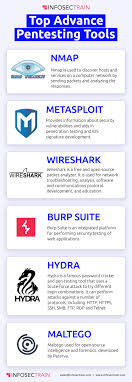
\includegraphics[height=0.3\textheight]{pentest_tools.jpg}
    \caption[Meest geavanceerde open source pentesting tools]{Meest geavanceerde open source pentesting tools}
  \end{figure}
Doelstelling: Dit hoofdstuk heeft als doel om duidelijk de criteria te definiëren die zullen worden gebruikt om de 
penetratietesttools te selecteren. Deze criteria zijn cruciaal om te garanderen dat de geselecteerde tools geschikt 
zijn voor onze specifieke testbehoeften en doelstellingen.

Deliverables:
\begin{itemize}
    \item Een gedetailleerde lijst van functionele en technische vereisten die elke tool moet voldoen.
    \item Een beoordelingskader dat zal helpen bij het evalueren en vergelijken van de tools op basis van deze vereisten.
\end{itemize}

Methoden:
\begin{itemize}
    \item Literatuuronderzoek: Bestudering van bestaande literatuur over penetratietesttools en -methodologieën om een gefundeerde basis van vereisten op te stellen.
    \item Analyse van Best Practices: Onderzoek naar de standaarden en praktijken in de industrie die de benchmark vormen voor goede penetratietesting.
\end{itemize}

Verantwoording: De keuze voor deze methoden zorgt voor een grondige en breed onderbouwde set van criteria die niet alleen theoretisch 
goed gefundeerd zijn maar ook industrieel relevant.

\section{\IfLanguageName{dutch}{Selectie van Geschikte Tools}{Selection of fitting tools}}
Doelstelling: Dit hoofdstuk focust op het proces van het selecteren van de meest geschikte penetratietesttool uit een 
bredere lijst. De geselecteerde tools worden geëvalueerd op basis van de vastgestelde criteria.

Deliverables:
\begin{itemize}
    \item een pentest tool die voldoet aan de vastgestelde criteria.
    \item Een evaluatierapport dat de beslissingsmatrix uitlegt en hoe elke tool zich verhoudt tot de vastgestelde criteria.
\end{itemize}

Methoden:
\begin{itemize}
    \item Vergelijkende Analyse: Evaluatie van elke tool op basis van de vereisten uit de requirements analyse.
    \item Scoringsmodel: Ontwikkeling van een kwantitatief model dat scores toekent aan elke tool op basis van de mate waarin zij aan de criteria voldoen.
    \item Feedbacksessies: Overleg met stakeholders en experts om de voorlopige selectie te verfijnen en te valideren.
\end{itemize}

Verantwoording: Deze stap zorgt voor een objectieve en transparante keuze van tools, wat essentieel is voor de 
geloofwaardigheid en bruikbaarheid van de uiteindelijke onderzoeksresultaten.

\section{\IfLanguageName{dutch}{Analyse van resultaten}{Analysis of results}}
Doelstelling: Analyse van de testresultaten om inzicht te verkrijgen in de effectiviteit van elke geselecteerde tool in het 
identificeren van kwetsbaarheden binnen de verschillende webomgevingen.

Deliverables:
\begin{itemize}
    \item Een uitgebreid analyserapport dat gedetailleerde bevindingen bevat over de prestaties van elke tool.
    \item Grafieken en tabellen die de resultaten visualiseren en vergelijken.
    \item Aanbevelingen voor de inzet van specifieke tools gebaseerd op de geteste prestaties.
\end{itemize}

Methoden:
\begin{itemize}
    \item Data-analyse: Verwerking en analyse van de verzamelde gegevens met behulp van statistische software om patronen en significante resultaten te identificeren.
    \item Kwalitatieve Beoordeling: Beoordeling van de aard en ernst van de gedetecteerde kwetsbaarheden door de verschillende tools.
    \item Vergelijkende Evaluatie: Systematische vergelijking van de resultaten om de relatieve sterktes en zwaktes van elke tool te bepalen.
\end{itemize}

Verantwoording: Deze analytische aanpak biedt een grondige en diepgaande evaluatie van de verzamelde data, waardoor sterke, 
data-gedreven aanbevelingen mogelijk zijn die de beveiligingspraktijken binnen de geteste omgevingen kunnen verbeteren.